\section{The Lazart tool}

\subsection{Lazart and robustness evaluation tools}

\begin{frame}[fragile]{Lazart}
\vfill
{\small

    \begin{figure}
        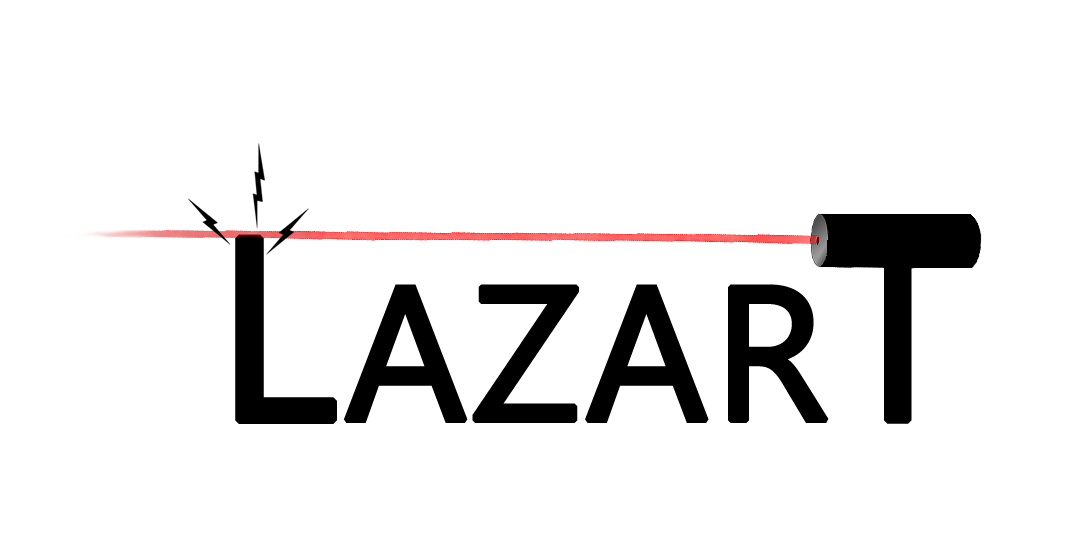
\includegraphics[scale=0.21]{img/lazart-logo-red.png}
    \end{figure}
    
    Lazart \cite{potet2014lazart} is an LLVM-level multi-fault robustness evaluation tool based on Dynamic-Symbolic Execution (KLEE)
    \begin{itemize}
        \item[] $\rightarrow$ Help developer to develop secure code
        \item[] $\rightarrow$ Help auditor to find vulnerabilities
        \item[] $\rightarrow$ Help for evaluation of countermeasures schemes
    \end{itemize}

    \vspace{0.8cm}
    
    \begin{columns}
        \begin{column}{0.5\textwidth}
            \onslide<2->{   \textbf{Handling multiple faults}:
                \begin{itemize}
                    \item Support for fault models combination
                    \item Fine description of fault space
                    \item Notion of redundancy and equivalence
                    \item[] 
                \end{itemize}
            }
        \end{column}
        \begin{column}{0.5\textwidth} 
            \onslide<3->{\textbf{Fault models}
                \begin{itemize}
                    \item Test/Branch inversion
                    \item Data mutation (\texttt{load}) (symbolic)
                    \item Jump (user-defined)
                \end{itemize}
                $\rightarrow$ cover most of high-level fault models
            }
            \vfill
    
        \end{column}
    \end{columns}
}
\end{frame}



\subsection{Principles}

\begin{frame}[fragile]{DSE and Fault Injection attacks}
\vfill
{\small

    An \textit{Injection Point} (IP) is mutated using a \textit{symbolic boolean} determining if an injection occurs, forking execution into the nominal and faulted behavior
 
    \begin{columns}   
        \begin{column}{0.5\textwidth}
            \lstset{language=C,style=customc, caption={Nominal behavior},label=lst:symbolic-ip-nominal, showlines=true}
            \begin{lstlisting}7
normal_behavior()






            \end{lstlisting}  
        \end{column}
        \begin{column}{0.5\textwidth}
            \lstset{language=C,style=customc, caption={Fault behavior},label=lst:symbolic-ip-fault, escapeinside={(*}{*)}}
            \begin{lstlisting}[label=lst-symbool]
(*{\color{mauve}inject}*) = symbolic_bool()
if (*{\color{mauve}inject}*) (*{\color{dkgreen}and}*) (*{\color{mauve}\_fault\_count}*) <= 
        (*{\color{mauve}\_fault\_limit}*):
    (*{\color{mauve}\_fault\_count}*)++
    faulted_behavior()
else:
    normal_behavior()
            \end{lstlisting}  
        \end{column}
    \end{columns}

    \begin{itemize}
        \item[] Only faults (+ values) and some entries (user-defined) are symbolic
        \item[]
    \end{itemize}

    \onslide<2>{
        \begin{itemize}
            \item Dynamic Symbolic Execution = Symbolic Execution + concretization
            \item[] $\rightarrow$ \textit{correct} (except for some concretizations)
            \item[] $\rightarrow$ not guaranteed to be \textit{complete} on path enumeration
        \end{itemize}
        
        $\rightarrow$ Lazart tries to give as much information as possible (timeout, coverage, errors...)
    }
}
\end{frame}

\subsection{Lazart's analysis}

\begin{frame}[fragile] \frametitle{Attack analysis - \texttt{verify\_pin}}
{\small
    \begin{columns}
        \begin{column}{0.60\textwidth}
            \begin{itemize}
                \item Analysis parameters:
                \item[]
                \begin{itemize}
                	\item \textbf{Inputs}: Incorrect PIN
                	\item \textbf{Attack objective}: being authenticated with a false PIN
                	\item \textbf{Fault model}: up to N \textit{test inversions}
                 \item[]
                \end{itemize}
            \end{itemize}        
            
            \begin{center}
                \begin{table}[]
                    \begin{tabular}{|l|l|l|l|l|l|}
                    \hline
                    \rowcolor[HTML]{C0C0C0} 
                    Fault limit (N)                           & 0                         & 1                         & 2                         & 3                          & 4                          \\ \hline
                    \rowcolor[HTML]{FFCCC9} 
                    \cellcolor[HTML]{C0C0C0}Attacks & \cellcolor[HTML]{9AFF99}0 & 1                         & 5                         & 10  & 11                          \\ \hline
                    \end{tabular}
                \end{table}
            \end{center}

            \onslide<2->{
                \begin{itemize}
                    \item[]
                    \item A successful 2-order attack (right) inverts the loop's condition {\color{Red}i < size} and the later check \\{\color{Red}if(i != size) killcard();}
                    \item[]
                \end{itemize}
            }
            
            \onslide<3>{
                \begin{itemize}
                    \item [] $\rightarrow$ How to simplify the attacks presented to the user in multiple faults ?
                \end{itemize}
            }
        \end{column}
        
        \onslide<2->{
            \begin{column}{0.48\textwidth}
                \begin{figure}
                        \caption{The 2-faults attack (Test Inversion)}
                    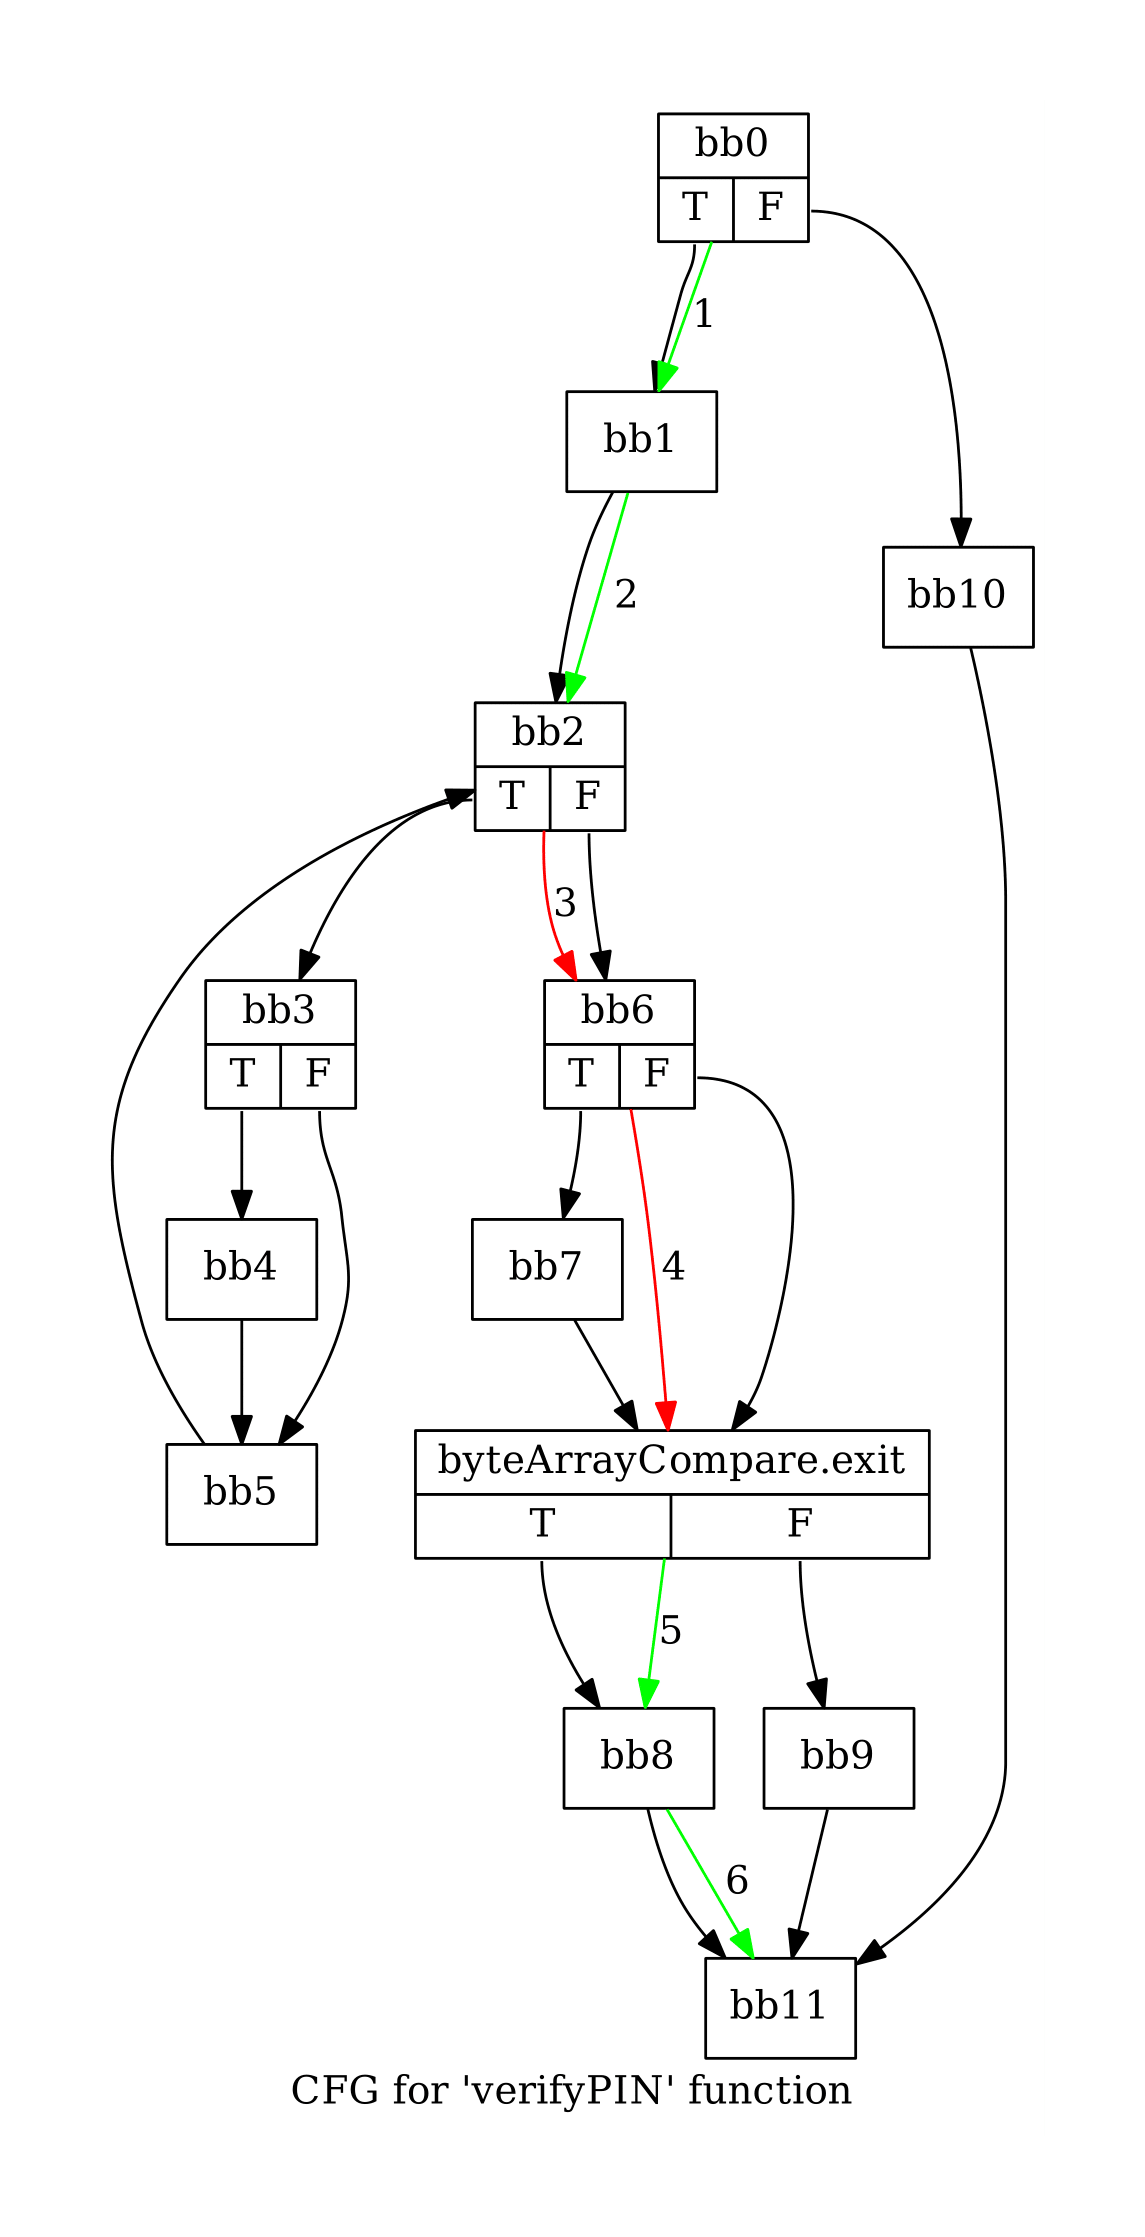
\includegraphics[scale=0.08]{img/o2-ti-atk.png}
                \end{figure}
            \end{column}
        }
        \end{columns}
    }
\vfill
\end{frame}

\begin{frame}[fragile]{Redundancy / Equivalence}
\vfill
{\tiny
    {\small Attack traces are represented as a sequence of \textit{nominal} and \textit{faulted} transitions}

    \only<1-2>{
        \begin{itemize}
            \item[]
            \item \textbf{Redundancy} and \textbf{equivalence} aims to filter attacks for the user in multiple faults
            \item[]
        \end{itemize}
    
        \begin{definition}[Redundancy prefix]
            An attack $a'$ is \textit{redundant by prefix} wrt an attack $a$ if the word of faulted transition of $a$ is a \textbf{proper prefix} of the faulted transition word of $a'$ 
        \end{definition}

        \begin{figure}
            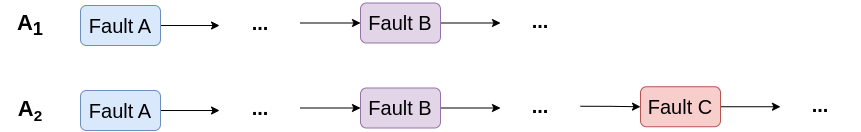
\includegraphics[scale=0.32]{img/red-prefix.png}
        \end{figure}
        \vfill
    }
    
    \only<2>{
        \begin{definition}[Redundancy subword]
            An attack $a'$ is \textit{redundant by subword} wrt an attack $a$ if the word of faulted transition of $a$ is a \textbf{strict subword} of the faulted transition word of $a'$ 
        \end{definition}
    
        \begin{figure}
            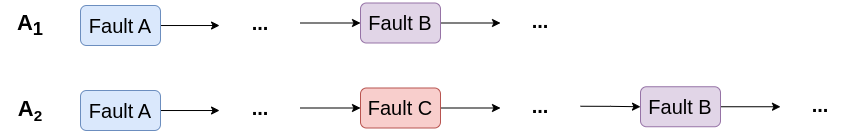
\includegraphics[scale=0.32]{img/red-subword.png}
        \end{figure}
        \vfill
    }

    \only<3>{
        \begin{itemize}
            \item[]
            \item \textbf{Redundancy} and \textbf{equivalence} aims to filter attacks for the user in multiple faults
            \item[]
        \end{itemize}
    
        \begin{definition}[Equivalence]
            An attack $a$ is \textbf{equivalent} to an attack $a'$ if their sequence of transitions are equal
        \end{definition}
    
        \begin{definition}[Fault-equivalence]
            An attack $a$ is \textbf{equivalent} to an attack $a'$ if their sequence of faulted transitions are equal
        \end{definition}
    
        \begin{figure}
            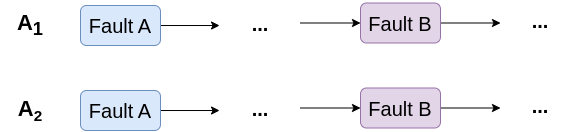
\includegraphics[scale=0.32]{img/red-min.drawio.png}
        \end{figure}
    }
\vfill
}
\end{frame}

\begin{frame}[fragile]{Experimentation}
\vfill
{\tiny
    \begin{columns}    
        \begin{column}{0.5\textwidth}
            Tested programs:
            \begin{itemize}
                \item \textit{Verify\_PIN} (\textbf{vp}): smart-card PIN verification process
                \item[] $\Rightarrow$ \textit{model}: test inversion
                \item \textit{RSA Cipher} (\textbf{rsa}): implementation of RSA encryption scheme. 
                \item[] $\Rightarrow$ \textit{model}: data load mutation
                \item \textit{Firmware Updater} (\textbf{fu}): updates a firmware from remote source
                \item[] $\Rightarrow$ \textit{models}: test inversion and data load mutation
            \end{itemize}
        \end{column}
        \begin{column}{0.5\textwidth}
            \onslide<2->{
                \begin{itemize}
                    \item Simplifies the number of attacks to consider
                    \item[] $\Rightarrow$ by a factor $200$ in a set of 15 examples from FISSC
                    \item[]
                    \item DSE is the main limit factor 
                    \item[] $\rightarrow$ with redundancy analysis matching on some examples
                \end{itemize}
            }    
        \end{column}
    \end{columns}

    \vspace{0.2cm}
    
    \onslide<2->{
        \begin{table}[p]            
            \caption{{\tiny Attack analysis on example programs}}\label{tbl:ch3:exp:fissc-results}
            \begin{center}
                \setlength\tabcolsep{4pt} % default value: 6pt
                \begin{tabular}{lll|lllll|lllll}
                \multicolumn{3}{l|}{Program} &  \multicolumn{5}{l|}{Attacks} & \multicolumn{5}{l}{Minimal attacks (with equivalence)}  \\
                Nom & LoCs & IPs &  1F & 2F & 3F & 4F & Total & 1F & 2F & 3F & 4F & Total \\
                \hline
                \hline
                vp0 & 25 & 4 &  12 & 21 & 18 & 7 & \textbf{58} & 3 & 0 & 0 & 0 & \textbf{3}  \\
                \hline
                vp4 & 45 & 11 &  34 & 118 & 180 & 147 & \textbf{479} & 3 & 0 & 1 & 0 & \textbf{4}  \\
                \hline
                vp7 & 78 & 8 &  4 & 36 & 116 & 173 & \textbf{329} & 1 & 2 & 0 & 0 & \textbf{3}  \\
                \hline
                rsa0 & 65 & 15 &  7 & 37 & 151 & 425 & \textbf{620} & 7 & 0 & 0 & 0 & \textbf{7}  \\
                \hline
                fu1 & 93 & 23  &  1 & 72 & 915 & 8191 & \textbf{9179} & 1 & 8 & 9 & 13 & \textbf{31}  \\
                \hline
                fu2  & 126 & 7  &  17 & 119 & 425 & 1031 & \textbf{1592} & 17 & 2 & 10 & 53 & \textbf{82}  \\
                \hline
                \hline
                \end{tabular}
            \end{center}
        \end{table} 
    }
}
\end{frame}


\begin{frame}[fragile]{Summary}
\vfill
{\small        
    My contributions:
    \begin{itemize}        
        \only<1>{
            \item \textbf{Python API :}
            \begin{itemize}
                \item \textbf{Manipulation of traces, analysis and models}
                \item \textbf{Fine fault space specification}
                \item \textbf{User accessibility: error handling, control on attack objective}
            \end{itemize}
        }
        \onslide<2->{
            \item Python API
            \begin{itemize}
                \item Manipulation of traces, analysis and models
                \item Fine fault space specification
                \item User accessibility: error handling, control on attack objective
            \end{itemize}
        }
        \only<2>{
            \item \textbf{Rewriting of Wolverine (mutation tool):}
            \begin{itemize}
                \item \textbf{Fault model combination}
                \item \textbf{Models data (+symbolic) and jump}
                \item \textbf{Automated countermeasures (TM, LM..)}
                \item \textbf{Switch to LLVM 9 (KLEE 2)}
            \end{itemize}
        }
        \onslide<3->{
            \item Rewriting of Wolverine (mutation tool):
            \begin{itemize}
                \item Fault model combination
                \item Models data (+symbolic) and jump
                \item Automated countermeasures (TM, LM..)
                \item Switch to LLVM 9 (KLEE 2)
            \end{itemize}
        }   
        \only<3>{      
            \item \textbf{Analysis:}
            \begin{itemize}
                \item \textbf{Redundancy / Equivalence}
                \item \textbf{Hotspots analysis}
                \item \textbf{Countermeasure analysis}
            \end{itemize}
        }
        \onslide<4->{
            \item Analysis:
            \begin{itemize}
                \item Redundancy / Equivalence
                \item Hotspots analysis
                \item Countermeasure analysis
            \end{itemize}
        }
        \onslide<4->{
            \item \textbf{Combination of Lazart with static analysis (Frama-C) on Wookey boot loader [Lacombe 2023]}
            \item \textbf{Filed at APP}
        }
    \end{itemize}
}        
\vfill
\end{frame}
